\chapter{BATMAN Protocol}
\label{appendix_batman}
This appendix contains some additional details about the BATMAN ad hoc routing protocol.

\section{Originator Message (OGM) Format}
The core algorithm in the BATMAN protocol as well as its implementation have gone through several evolutionary changes during development. Currently the BATMAN developers are working on a version V of the protocol where they aim to improve issues such as mesh bonding, weighted Link Quality (LQ) measurements and multicast optimizations \cite{open_mesh_v}.
\\\\
During development there has also been some changes to the Originator Message (OGM) format. Figure \ref{fig:ogm} shown in Section \ref{batman} is the OGM as it is described in the Internet-Draft \cite{batman_rfc}. Two fields, Previous Sender Address and Transmit Quality (TQ), have been added to the OGM as shown in Figure \ref{fig:app_ogm}.
\\\\
A BATMAN packet consisting of an Originator Message (OGM) together with zero or more HNA extension messages, is encapsulated in a single UDP data packet. The format of the OGM is shown in Figure \ref{fig:app_ogm}.

\begin{figure}[ht]
	\centering
		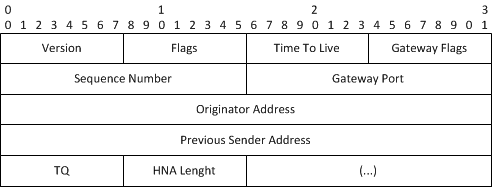
\includegraphics{images/ogm_v2.png}
	\caption{Originator Message (OGM) Format.}
	\label{fig:app_ogm}
\end{figure}

\noindent
The different fields in the OGM is explained below:
\\\\
\textbf{Version} \\
Identifies the version of BATMAN for the contained message
\\\\
\textbf{Is-direct-link flag} \\
Flag indicating whether a node is a direct neighbor or not.
\\\\
\textbf{Unidirectional flag} \\
Flag indicating whether the neighboring node is bidirectional or not.
\\\\
\textbf{Time To Live} \\
Contains the maximum number of hops a message will be transmitted.
\\\\
\textbf{Gateway Flags} \\
Indicates whether a node may act as a gateway with access to the Internet. 
\\\\
\textbf{Sequence Number} \\
Number added by an Originator to every OGM it broadcasts. Number is incremented for each OGM broadcasted.
\\\\
\textbf{Originator Address} \\ 
The IPv4 address of the B.A.T.M.A.N. interface on which behalf the OGM has been generated.


\subsection{Host Network Annoncement Message Format}
The Host Network Announcement (HNA) is used to announce that a node is a gateway to another network. If so, the node sets the Gateway Flag in the OGM and appends a HNA-extension-message containing the netmask and the network address of the announced network.
\\\\
HNA-extension-message format is shown in Figure \ref{fig:app_hna}.

\begin{figure}[ht]
	\centering
		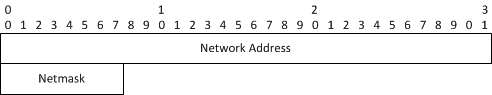
\includegraphics{images/hna.png}
	\caption{Host Network Announcement Message format.}
	\label{fig:app_hna}
\end{figure}


